\documentclass[11pt, a4paper]{article}

\usepackage[utf8]{inputenc}
\usepackage[T1]{fontenc}
\usepackage[polish]{babel}
\usepackage{amsmath}
\usepackage{amsfonts}
\usepackage{graphicx}
\usepackage{geometry}
\usepackage{listings}
\usepackage{xcolor}
\usepackage{float}

\geometry{
    a4paper,
    total={170mm,257mm},
    left=20mm,
    top=20mm,
}

% Konfiguracja formatowania kodu Python
\definecolor{codegreen}{rgb}{0,0.6,0}
\definecolor{codegray}{rgb}{0.5,0.5,0.5}
\definecolor{codepurple}{rgb}{0.58,0,0.82}
\definecolor{backcolour}{rgb}{0.95,0.95,0.92}

\lstdefinestyle{mystyle}{
    backgroundcolor=\color{backcolour},   
    commentstyle=\color{codegreen},
    keywordstyle=\color{magenta},
    numberstyle=\tiny\color{codegray},
    stringstyle=\color{codepurple},
    basicstyle=\ttfamily\footnotesize,
    breakatwhitespace=false,         
    breaklines=true,                 
    captionpos=b,                    
    keepspaces=true,                 
    numbers=left,                    
    numbersep=5pt,                  
    showspaces=false,                
    showstringspaces=false,
    showtabs=false,                  
    tabsize=2
}
\lstset{style=mystyle}

\title{\textbf{Podstawy Symulacji Komputerowej} \\ Lista 1 zadanie 2}
\author{}
\date{}

\begin{document}

\maketitle

\section*{Treść zadania}
Napisać program wykonujący algorytm kwadratowy von Neumanna.

\section*{Opis metody}
Algorytm środka kwadratu (zaproponowany przez Johna von Neumanna) to jedna z najstarszych metod generowania liczb pseudolosowych. Metoda opiera się na następujących krokach:
\begin{enumerate}
    \item Wybór początkowej wartości ziarna (ang. \textit{seed}) o długości $n$ cyfr.
    \item Podniesienie tej wartości do kwadratu, co daje liczbę o długości do $2n$ cyfr.
    \item Uzupełnienie wyniku zerami wiodącymi (jeśli to konieczne), aby zachować stałą długość $2n$.
    \item Wyciągnięcie $n$ środkowych cyfr, które stają się kolejną wygenerowaną liczbą i nowym ziarnem dla następnej iteracji.
\end{enumerate}
Częstym problemem tego algorytmu jest szybkie zapętlanie się lub zbieganie do zera. W poniższej implementacji wprowadzono mechanizm zapobiegający temu zjawisku poprzez resetowanie wartości w przypadku osiągnięcia zera.

\section*{Implementacja}
Symulację wykonano w języku Python. Poniżej przedstawiono implementację generatora oraz funkcji wizualizujących niezależność wygenerowanych próbek w przestrzeni 2D i 3D:

\begin{lstlisting}[language=Python, caption=Implementacja algorytmu kwadratowego von Neumanna]
import matplotlib.pyplot as plt

def von_neumann_generator(seed, n_samples):
    current = seed
    results = []
    
    for i in range(n_samples):
        # Podniesienie do kwadratu i wyrownanie do 8 znakow
        square_str = str(current**2).zfill(8)
        
        # Pobranie 4 srodkowych cyfr (indeksy 2,3,4,5)
        middle_str = square_str[2:6]
        current = int(middle_str)
        
        # Normalizacja do przedzialu [0, 1)
        results.append(current / 10000.0)
        
        # Zabezpieczenie przed utknieciem w zerze
        if current == 0:
            current = 1234 + i 
            
    return results

def plot_2d_independence(data):
    x = data[:-1]
    y = data[1:]
    
    plt.figure(figsize=(8, 8))
    plt.scatter(x, y, alpha=0.6, s=15, color='blue')
    plt.title("Test graficzny 2D: Von Neumann ($r_n$ vs $r_{n+1}$)")
    plt.xlabel("$r_n$")
    plt.ylabel("$r_{n+1}$")
    plt.grid(True, linestyle='--', alpha=0.5)
    plt.show()

def plot_3d_independence(data):
    # Tworzymy trojki (x, y, z)
    x = data[:-2]
    y = data[1:-1]
    z = data[2:]
    
    fig = plt.figure(figsize=(10, 8))
    ax = fig.add_subplot(111, projection='3d')
    
    ax.scatter(x, y, z, alpha=0.6, s=10, color='purple')
    ax.set_title("Test graficzny 3D: Von Neumann ($r_n, r_{n+1}, r_{n+2}$)")
    ax.set_xlabel("$r_n$")
    ax.set_ylabel("$r_{n+1}$")
    ax.set_zlabel("$r_{n+2}$")
    plt.show()
    
# Wykonanie algorytmu
samples = von_neumann_generator(seed=1234, n_samples=500)
\end{lstlisting}

\section*{Wyniki symulacji i testy graficzne}
Wygenerowano próbkę $N = 500$ liczb pseudolosowych dla początkowego ziarna $1234$. 
Pierwsze wartości wygenerowanego ciągu to m.in.: $0.5227, 0.3215, 0.0336, 0.1128$.

Aby sprawdzić jakość wygenerowanego ciągu i niezależność kolejnych próbek, przeprowadzono testy graficzne w wymiarze 2D (punkty o współrzędnych $r_n, r_{n+1}$) oraz 3D (punkty o współrzędnych $r_n, r_{n+1}, r_{n+2}$).

\begin{figure}[H]
    \centering
    % Odkomentuj ponizsza linie i upewnij sie, ze masz plik wykres2d.png
    % 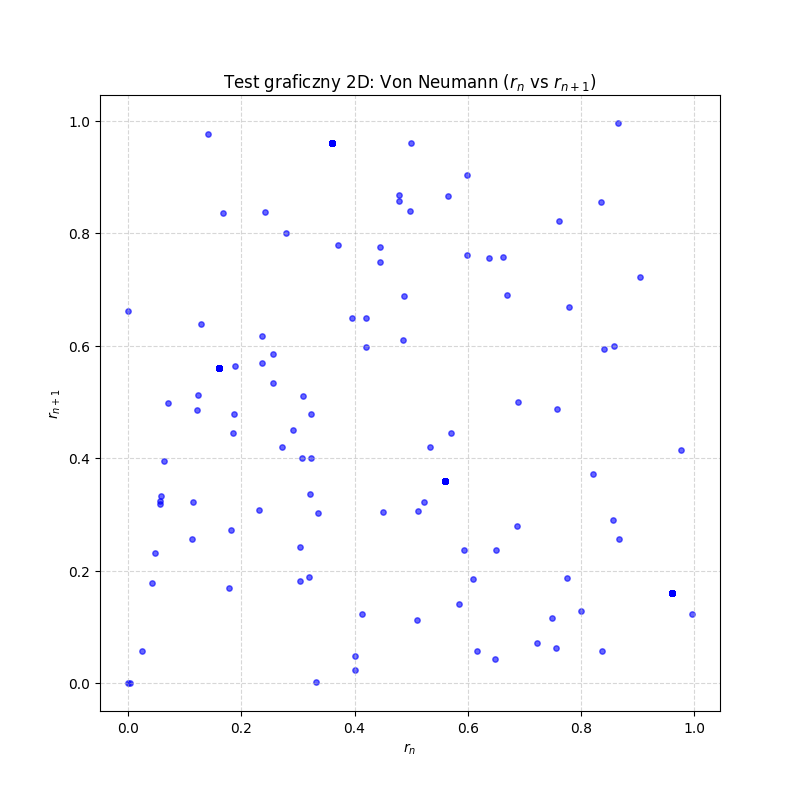
\includegraphics[width=0.8\textwidth]{wykres2d.png}
    \vspace{5cm} % Usun to \vspace gdy dodasz grafike
    \caption{Rozkład par $(r_n, r_{n+1})$ w teście 2D.}
\end{figure}

\begin{figure}[H]
    \centering
    % Odkomentuj ponizsza linie i upewnij sie, ze masz plik wykres3d.png
    % 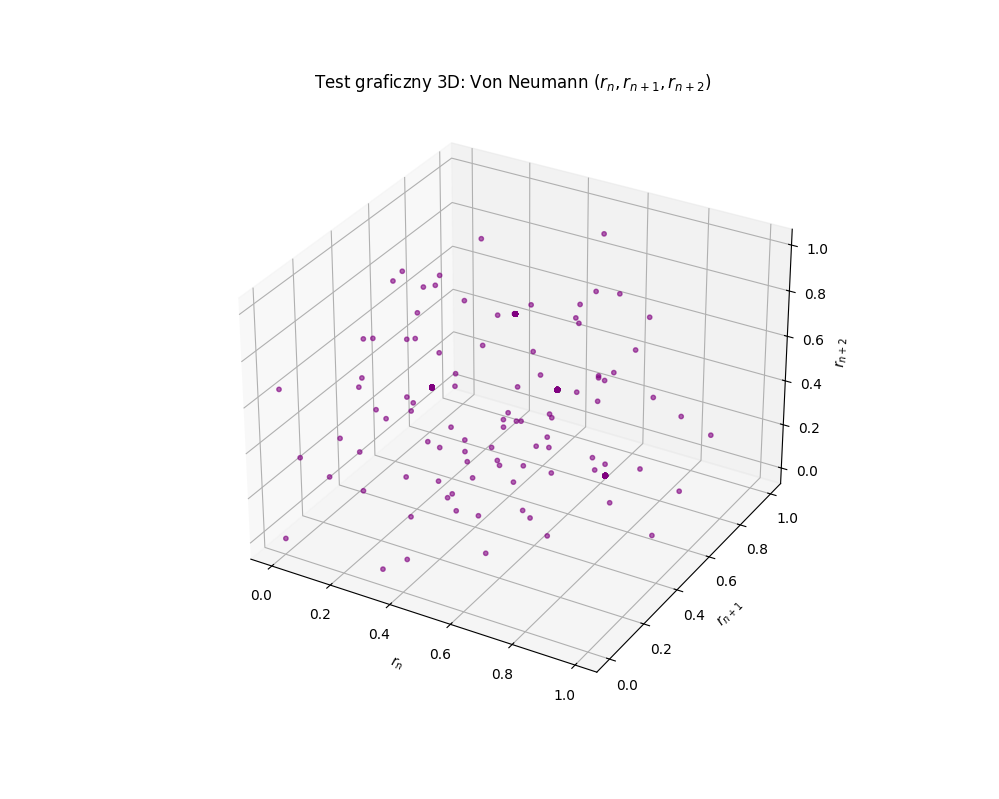
\includegraphics[width=0.8\textwidth]{wykres3d.png}
    \vspace{5cm} % Usun to \vspace gdy dodasz grafike
    \caption{Rozkład trójek $(r_n, r_{n+1}, r_{n+2})$ w teście 3D.}
\end{figure}

\section*{Interpretacja wyników}
Na podstawie przeprowadzonych testów graficznych (wykresy 2D i 3D) można wstępnie ocenić jakość generatora. Zbyt wyraźne wzory, prążki lub skupiska punktów na wykresach świadczyłyby o silnej zależności między kolejnymi próbkami, co jest charakterystyczną wadą prostych generatorów (takich jak klasyczny algorytm von Neumanna). Zastosowane w kodzie zabezpieczenie (zmiana stanu przy wygenerowaniu $0$) zapobiega całkowitej degradacji ciągu, jednak dla profesjonalnych zastosowań symulacyjnych metoda ta ustępuje nowoczesnym generatorom.

\end{document}